\section{Motivation}

The FINken project aims at creating a swarm of autonomously flying quadcopters to research swarm intelligence behaviour on robots.
Many algorithms in swarm intelligence are based on distance values.
As a consequence it is important to find a sensor that is capable of measuring distances between copters and to integrate it into the FINken robots.
An obvious choice for this distance function is measuring the euclidian distance in between the robots.

There are already ranging sensors that are incorporated into the FINken robots.
However, those sensors measure the distance to arbitrary objects in the environment.
The new sensor should be able to measure the distance to another sensor which is queried by address.

\section{Requirements}
\label{req}
There are basically three requirements for the ranging sensor.
Fulfilling these requirements is the goal of this thesis.

\begin{enumerate}
	\item Interaction between the copter and the ranging modules should be minimal.
	\item The ranging nodes need to be integrated into the copter.
	\item The values yielded by ranging should be of usable quality.
\end{enumerate}

\subsection{Interaction between Copter and Ranging}
\label{req1}
The copter should not influence the function of the ranging modules and vice versa.
Using an ultrasonic ranging method might not be feasible as the copter already uses multiple ultrasonic sensors.
If no measures are taken to counteract medium access problems, both sensors will disrupt each other until the sensor values of both sensors are completely useless.

This requirement can be mitigated to a certain degree.
If there is interaction between copter and ranging sensors, the setup of the quadcopter could be changed to eliminate the interaction.
However, the FINken robot is used in research and changing one component usually means almost all components have to be adjusted, as most components are interdependable to some degree.

\subsection{Integration of the Ranging Modules}
\label{req2}
In order to be used in the FINken project, the sensors need to be integrated into the robots.
This means that the ranging modules need to be lightweight and small enough to fit on a flying robot.
Additionally, there needs to be an interface that can transmit the data from the new sensor to the firmware controlling the robot.

One of the aspects of integration is that the robots should interact locally to form a swarm\footnote{
In contrast to a multi agent system that would rely on a common knowledge base.}.
As a consequence, it is not sufficient to measure the positions of the copters with external sensors and to provide the distance values via telemetry. The robots should rely solely on internal sensors.

\subsection{Yielding Usefull Values}
\label{req3}
Yielding usefull values seems to be a trivial requirement, but is actually the hardest of all three.
The area of operation for the FINken robots is only \SI{3}{m} wide and \SI{4}{m} long so the range measurements need to be sufficiently accurate for those small distances.

It is desireable that the range measurements fulfill the properties of a distance function.

Additionally, the update frequency needs to be high enough to support the great accelarations and velocities of the FINken robots.


\section{The FINken Robot Platform}


The goal of the FINken project is to implement intelligent swarm behaviour on flying robots and to research how swarm collaboration performs in a real world application.
The robots need to fly in an stable manner on their own and be capable of interacting with other other.
Nevertheless, they must not disrupt the other swarm members.
Those robots should perform given tasks defined to encourage swarm based interaction.
Their behaviour can be evaluated and compared to the theoretical models developed by swarm intelligence research.

\subsection{Robot Description}

The robots are propelled by four rotors that are driven by brushless motors.
The quadcopter is rotated around pitch, roll and yaw axis by controlling the motors.
Additionally, the overall amount of thrust can be changed.
The airframe houses all the actuators, processors and batteries needed for flight.
It carries a multitude of sensors used for operating autonomously and interacting with other robots and the environment.

\begin{figure}[H]
	\centering
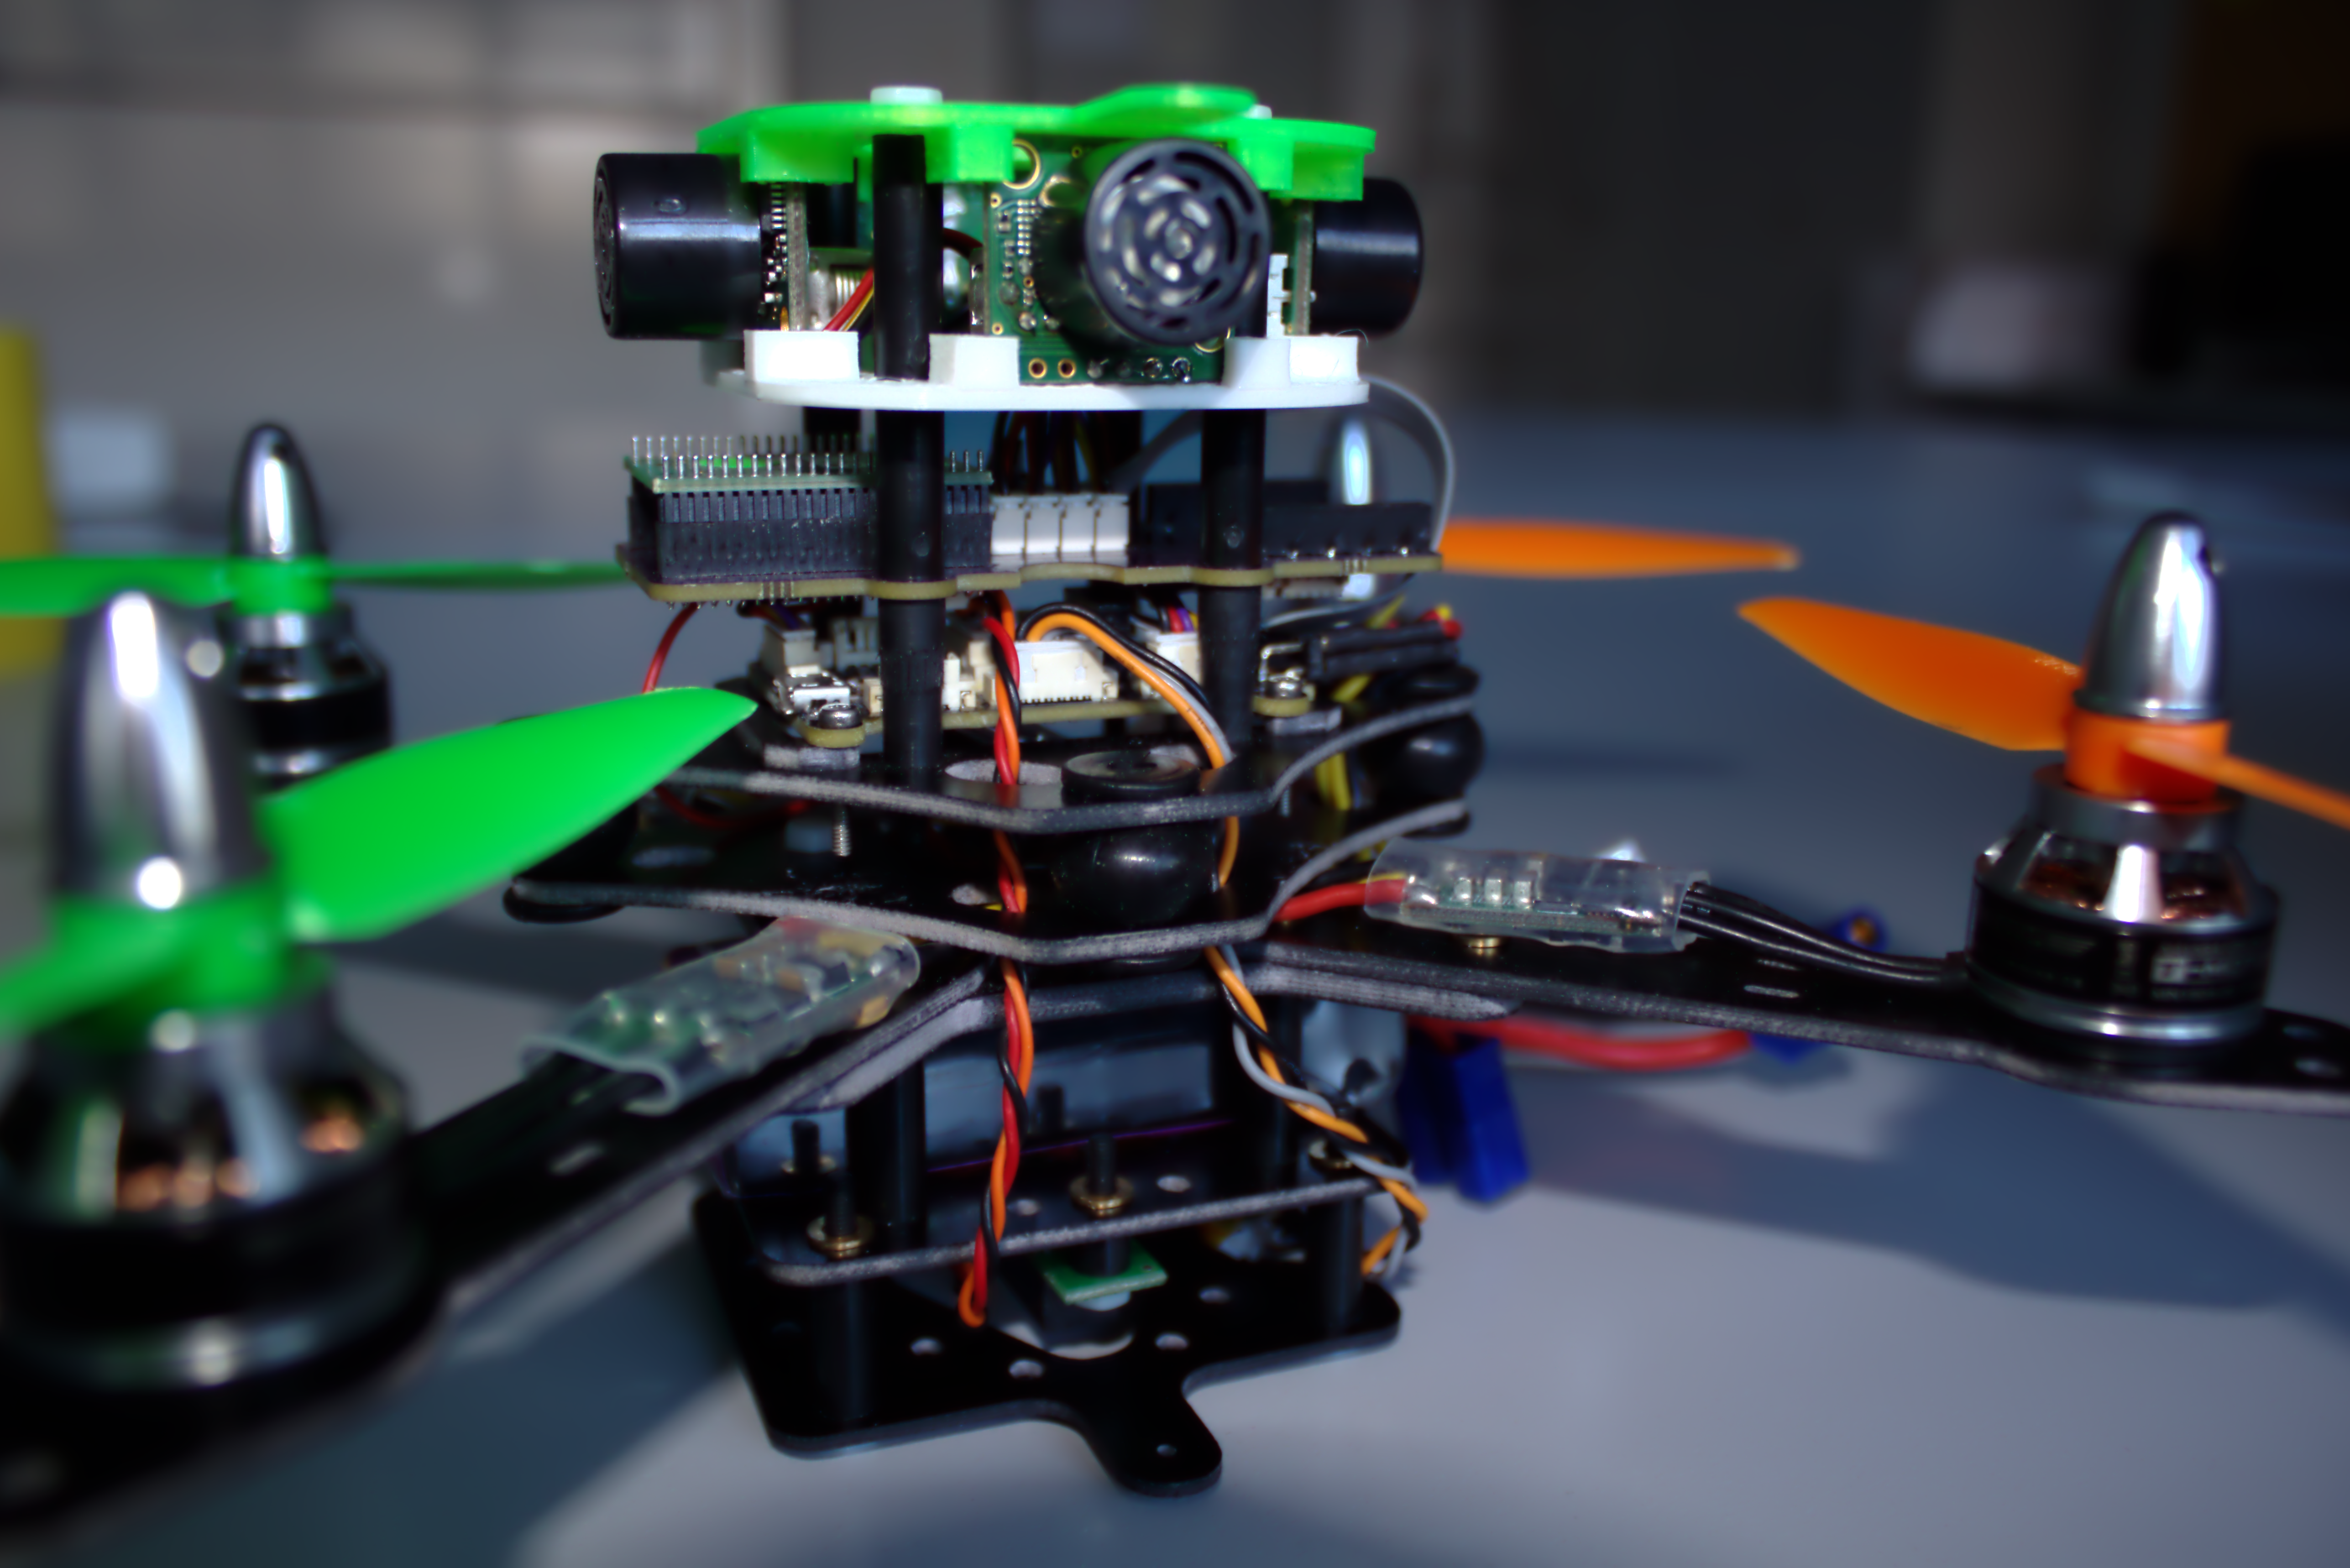
\includegraphics[width=0.9\textwidth]{figures/copter.png}
\label{copterfoto}
\caption{The FINken robot, revision 3}
\end{figure}

The robots are capable of highly dynamic flight maneuvers—the robots have enough acceleration to leave the operating environment in any possible direction in less than one second.
This is mainly because the robots need lots of payload capacity to carry different sensors.
However, highly dynamic behaviour is not usefull for our research.
The high power of the motors can also be used to better stabilise the copter, which is needed for the FINken research.

The FINken robot needs to be controlled very accurately.
If the copter is angled by only $3\degree$ and its height is kept stable, it is accelerating at about \SI{1}{\metre\per\square\second}.
The copter reaches a velocity of over \SI{1}{\metre\per\second} when travelling through the arena at this small angle.
The example illustrates why the algorithms controlling the copter are susceptible, even to small calibration offsets in pitch and roll angle.

\subsection{Environment}
\label{env}
The FINken project is focused solely on indoor application.
Special characteristics of indoor flight are the following:
\begin{itemize}
	\item The area of operation is small and enclosed.
	\item Some sensors\footnote{ In particular GPS, magnetometer and barometer. } that are typically used in quadcopters are not suited for indoor use.
	\item Velocities are much lower.
	\item Miniaturisation becomes a necessity.
	\item Humans need to be protected from the quadcopters.
\end{itemize}

In the swarmlab the quadcopters fly in an enclosed arena.
It is designed to protect the robots from mechanical damage.
Furthermore, it will not disrupt the function of the sensors the robot is using.

The FINken robots fly in an area of \SI{2}{\metre} by \SI{3}{\metre} that can be expanded to about \SI{3}{\metre} by \SI{4}{\metre}.
The flight area is enclosed by netting and ultrasound-reflecting foil.
Those barriers act the same way a wall would do, without damaging the robots if they fail to elude them.
Usually, the altitude of operation is between \SI{0.4}{\metre} to \SI{1}{\metre}.
To prevent damage when the quadcopters crash, the floor is covered with mats that work well with ultrasound and infrared sensors used by the FINken.

Additionally, a projector creates artifical environmental factors for the robots by projecting an image into the arena.
The colour at the current position can be measured by an rgb-sensor mounted on top of the robots.
Certain tasks may be assigned to the robots to interact with this environment, for example finding the brightest spot.
The advantage of this method is that this environment is easy reproduce and change.


\subsection{Sensor Concept}
The sensors used by the FINken robots serve two purposes: To enable the robots to fly autonomously and to interact with other robots and the environment.

The robots need to function as single individuals to form a swarm.
That means not crashing into walls, ceiling, floor or other robots.
The sensors needed to achieve this behaviour are more important than the other sensors of the quadcopter.

Not crashing breaks down into two major problems: Height control and navigating the x-y-plane without colliding with other physical objects.

\subsubsection*{Height Control}

To control the height of the copter a sensor is needed that is able to measure the current altitude.
Two sensors are capable of this measurement: The IR-sensor and the optical flow sensor\footnote{The actual height measurement is made by an ultrasonic distance sensor that is one compontent of the optical flow sensor}.
Each of these sensors is sufficient for height control on its own, usually only one of both sensors is installed.

\subsubsection*{Detecting Physical Objects}

To detect physical objects in its vicinity the FINken is equipped with four ultrasonic distance sensors.
With those sensors objects cannot be differentiated.
The nearest object in the direction of perception is sensed.

The ultrasonic sensors allow the robot to evade walls and other obstacles by keeping a safe distance.

\subsubsection*{Interaction With Other Quadcopters}

The ultrasound sensors are also used to avoid collsions with other quadcopters.
Additionally, the new ranging sensor can be utilised to allow more complex interactions between copters as the range sensors can distinguish between the copters and other ranging nodes.

\subsubsection*{Measuring Speed}

With both height control and wall avoidance the FINken are capable of flying for long time periods.
This works as long as the velocity of the robot is small enough so it is able to react to obstacles in time.
The optical flow sensor is currently utilised to restrict the movement speed of the copter. 
This is another possible field of application for the range sensors.

In the small operating area in the swarmlab the velocities are usually not exceeded.
For this reason the optical flow sensor is not mandatory.

\subsubsection*{Interaction With a Virtual Environment}

To research interaction with an artifical environment as described in \autoref{env} the quadcopters are equipped with a colour-sensor.
Similarly the ranging sensor can be used to create virtual points of interest that can be sensed by the robots.

\subsubsection*{Orientation}

The quadcopters only navigate based on their current perception, in particular by following the walls.
Range measurements may be used for more sophisticated orientation strategies.
The copters could navigate by following beacons in the environment or by computing a position estimate.

\subsection{Hardware Description}
There are different ranging technologies that might be used in a FINken quadcopter.
However, different components can interfere with the new sensor.

\begin{table}[h]
	\begin{tabularx}{\columnwidth}{l | X}
	Part & Description \\ \hline
	Frame & The frame is made of GFK material and plastic, rotor to rotor distance is \SI{10}{\centi\metre} \\
	Propellers & The FINken use \SI{5}{"}x\SI{3}{"} propellers \\
	Motors & Four brushless motors that may cause RF-interference and noise \\
	Power-Supply & Lithium polymer batteries with nominally \SI{11.1}{\volt} output voltage that is converted to 5V and 3.3V by the power distribution hardware \\
	Sonar Sensors & Sonar sensors to measure the distances to the nearest object in four directions (front, back, left, right) \\
	Optical Flow & PX4 optical flow sensor to measure x- and y- velocity and distance to ground \\
	IR-Sensor & IR-distance sensor measuring distance to ground, alternativ to optical flow sensor \\
	Telemetry & BTLE-/Zigbee modules to exchange data with the ground station \\
	RC &  2.4GHz based radio control to manually control the robots \\
	Autopilot & Lisa/MX version 2.1~\cite{lisamx} running the paparazzi~\cite{paparazzi} autopilot firmware.
	\end{tabularx}
	\caption{Hardware Components of the FIKen 3 Robots}
\end{table}

\section{Evaluation of Existing Ranging Solutions}

Keeping the requirements from \autoref{req} in mind, there are some technologies that can be used for ranging.
The usual application for most of those technologies in research is positioning, which makes it difficult to find comparable numbers for ranging-only applications.
In positioning usually more than four range measurements are combined to compute one position.
By doing so ranging errors are mitigated to some degree.
When only doing ranging this method of error mitigation is not available.

It is still interesting to search for positioning applications, since many of those positioning technologies are based on multilateration\footnote{
The usual methods for positioning are: \emph{multilateral}—which is relevant for this work, because only ranging measurments are used. \emph{Multiangular}—where angle measurements are used and \emph{orientating in a map} with different factors like beacon-positions.}.
\cite{_multilateration_2015}

\subsection{Optical Tracking}
Most projects use external optical tracking to measure the position and orientation of the quadcopters. \todo{refs}

The most common optical tracking systems are very costly in comparison to the other ranging methods described here.
The most affordable solution from Optitrack able to track five targets at once costs more then \SI{10000}{\$}~\cite{optitrack.com}.
The price is justified by the superior performance of this method.
Optical tracking is highly accurate at a very high update frequency.
Additionally, it is able to measure the orientation of the quadcopters.
\todo{research performance statistics for ranging solutions}

\todo{ETH}

Even a tracking system that is more cost efficient such as the one developed by Achtelik et al\cite{Achtelik2009} is not an appropriate solution for the FINken project.
A tracking system provides information that is gathered for the entire operating area and afterwards broadcasted to the robots.
The big advantage of swarm behaviour would be lost.
No common information base is required in order to form a functioning swarm.

As such external tracking could be a valuable tool for observing the swarm behaviour.
However, it is not meeting the requirements for the sensor the robots should use (see \autoref{req2}).

%A huge drawback to this method is that many components are used that need to be integrated into the environment and cannot be carried by the robots themselves.
%For swarm robotics this is not an ideal solution as using external tracking would mean communicating with some kind of centralized tracking interface-destroying the scalability and the priciple of local interaction leading to global behaviour.

\subsection{Indoor Time of Flight}
An obvious approach for replacing the GPS signal is to use a similar approach indoors.

The problem is that very short timespans have to be measured accurately, because radio waves travel at the speed of light.
Lanzisera, Lin and Pister~\cite{lanzisera2006} state that standard errors of \SI{2.6}{\metre_{RMS}} and \SI{1.8}{\metre_{RMS}} were measured in different indoor scenarios.
With an operating area only \SI{3}{\metre} wide this solution is not suited for the robots.

A more promising project is DecaWave.
According to Kempke, Pannuto and Dutta~\cite{uwb_localisation_copter} the measurement error is generally less than \SI{1}{\metre} and with filtering can be brought to below \SI{15}{\centi\metre}.
Mahfouz et al\cite{uwb_decawave} even claims that an accuracy of \SI{10}{\centi\metre} can be achieved.
While the DecaWave modules seem like suitable ranging sensors for the FINken the hardware was not available to the FINken project at the time.

\subsection{Ultrasonic Time of Flight Ranging}
A very clever approach to ranging is used by ranging solutions like cricket~\cite{cricket_01} and active bat~\cite{active_bat}. 
RF-Signals travel at the speed of light and therefore very short time-periods need to be measured accurately to compute distances from time of flight.
Sound however travels at a speed much slower than radio waves so the time periods that need to be measured are much longer.
Unfortunately the slower propagation speed causes a different problem.

When using sound as medium there is an upper bound to the update frequency for all nodes sharing the medium. Woodman and Harle~\cite{active_bat} claim that one ranging measurement can be done in a \SI{20}{\milli\second} time slot.
As a result, there can be up to 50 range updates per second.
A swarm of five robots that form a fully connected graph would need at least ten range measurements to obtain all swarm distances.
So the upper boundary for ranging update frequency in this swarm of five robots is \SI{5}{\hertz}.
Considering that this is not the actual performance but the upper limit, this is a solid disadvantage of this method.

Currently the FINken robots use sonar based distance sensors to measure the distance to the nearby objects.
It is highly unlikely that those distance sensors and an ultrasonic ranging method can be used in parallel without disrupting each other.
This problem could only be solved by implementing some kind of medium access control protocol
By doing so the maximum update frequencys for both sensors would be reduced.


%Another problem is the noise created by motors and propellers.
%The sound made by the quadcopters is not ending in the hearable spectrum but also extends to the ultrasound range.
In conclusion, ultrasound based ranging is a very neat approach to ranging that is already used in other quadcopter projects~\cite{ultrasonic_erlangen}.
Still integrating an ultrasonic ranging sensor into the FINken is impractical, because other ultrasound sensors are already in use.
%\todo{accuracy / price, moving objects}


\subsection{Signal Strength}

A property that can be used to do RF-based ranging is signal strength.
The further the source of the signal is away the weaker the signal gets.
RSSI\footnote{Received Signal Strength Indicator}-based ranging is done for serveral different wireless technologies: Bluetooth\cite{pei_using_2010}, WLAN\cite{wlanrssi, wlanrssi2}, RFID\cite{rfidrssi}.

There are serveral drawbacks to RSSI based ranging. Zanca \cite{Zanca} writes: "Unfortunately, the indoor radio channel is very
unpredictable, since reflections of the signal against walls, floor and ceiling may result in severe multi–path interference at the receiving antenna.".
Furthermore, no antenna will transmit radio waves equally in every direction–especially if it is mounted on a robot containing lots of wiring.

Ultimately, the orientaion and location of the quadcopter might have a bigger impact on the RSSI value than the actual range has.
Thus an RSSI based ranging method will probably not yield sufficient results.
%The main factor that rules out RSSI-based ranging is that radio-waves are not propageted equally in every direction. \todo{typical propagation pattern picture}
%As a consequence the orientation of the antenna might have a much bigger impact on signal strength then the distance.
%Additionally, radio waves might be weakend when travelling through the FINken robots.


\subsection{Phase Difference}

Another thing that can be measured is phase shift~\cite{2_kluge_eggert_2009}.
This is utilised by the ranging hardware from Atmel.
Multiple frequencys are used to measure a phase difference.
As the wave length changes with different frequencys a distance can be computed from all of the measured phase differences.
\todo{quelle!}
Similar hardware using the same software stack is sold by \emph{Dresden Elektronik} and \emph{Meterionic}.

Using phase differences in radio waves mitigates the medium access problems of ultrasonic methods as well as the wave propagation problems of RSSI-based methods.
Therefore, it seems like a feasible approach for the FINken robots.

\todo{tabelle -> ranging methoden übersichtlich vergleichen}
